% !TeX root=teoriaprocesovtakac.tex
% !TeX encoding = UTF-8
% !TeX spellcheck = sk_SK
\section{Procesy v kyslíkovom konvertore}

\subsection{Chemické procesy}

Podstatou výroby ocele v kyslíkovom konvertore je oxidácia prvkov z kovonosnej vsádzky s kyslíkom fúkaným do konvertora. Oxidy týchto prvkov prechádzajú do trosky alebo odchádzajú vo forme konvertorového plynu. Intenzita oxidácie jednotlivých prvkov závisí od ich chemickej afinity ku kyslíku.
Oxidácia uhlíka je jedným z najdôležitejších procesov. Uhlík sa v kove počas
oceliarenského pochodu oxiduje vplyvom kyslíka najmä na \ce{CO} a čiastočne na \ce{CO2} podľa reakcií

\begin{equation}
\ce{C + 1/2O2 -> CO}
\end{equation}
\begin{equation}
\ce{C + O2 -> CO2}
\end{equation}

Mangán sa v konvertore oxiduje na \ce{MnO}

\begin{equation}
\ce{Mn + 1/2O2 -> MnO}
\end{equation}

Fosfor je v oceli nežiaduci a oxiduje sa na \ce{P2O5}

\begin{equation}
\ce{2P + 5/2O2 -> P2O5}
\end{equation}

Síra patrí medzi škodlivé prvky a prechádza do trosky vo forme \ce{CaS} na základe reakcie \ce{CaO}

\begin{equation}
\ce{CaO + MnS -> CaS + MnO}
\end{equation}

pričom \ce{MnS} vzniká podľa reakcie

\begin{equation}
\ce{Mn + S -> MnS}
\end{equation}

a síra taktiež odchádza aj vo forme plynu ako \ce{SO2}

\begin{equation}
\ce{S + O2 -> SO2}
\end{equation}

Kremík ma vysokú afinitu ku kyslíku, čiže sa ľahko oxiduje pričom vzniká \ce{SiO2}

\begin{equation}
\ce{Si + O2 -> SiO2}
\end{equation}

Potrebné je taktiež uvažovať aj straty železa vo forme \ce{FeO} a \ce{Fe2O3}

\begin{equation}
\ce{Fe + 1/2O2 -> FeO}
\end{equation}

\begin{equation}
\ce{2Fe + 3/2O2 -> Fe2O3}
\end{equation}

ktoré prechádzajú do trosky, resp. \ce{Fe2O3} odchádza v konvertorovom prachu. Kvapky kovového železa sa nachádzajú aj v troske.

Vzniknutý \ce{SiO2} prechádza do trosky ako \ce{2CaO.SiO2} podľa rovnice

\begin{equation}
\ce{SiO2 + 2CaO -> 2CaO.SiO2}
\end{equation}

a obdobne \ce{P2O5} prechádza do trosky ako \ce{3CaO.P2O5} podľa rovnice

\begin{equation}
\ce{P2O5 + 3CaO = 3CaO.P2O5}
\end{equation}

\cite{sprava2017}.

\newpage
\subsection{Elementárne procesy}

LD proces sa skladá z nasledujúcich elementárnych procesov:

\begin{enumerate}
	\item Vsádzka
	\item Nalievanie tekutého surového železa
	\item Fúkanie kyslíka a pridávanie troskotvorných a legujúcich prísad
	\item Vzorkovanie (zber dát, zaznamenávanie teploty)
	\item Odpich ocele
	\item Odpich trosky
\end{enumerate}

V moderných oceliarňach sa vyrobí cca 300t ocele v priebehu 30-40 minútového cyklu. Pre prispôsobenie akosti ocele a tvorbu trosky sa počas pochodu pridávajú rozličné prísady. Počas vsádzky a odpichu je konvertorová pec naklonená. Počas fúkania kyslíka má konvertor zvislú polohu.

V závislosti od miestnych prevádzkových podmienok, dostupnosti šrotu, vysokopecného železa a rozsahu predúpravy, je pri vsádzke 75 až 95 \% kovového náboja do konvertora LD/BOF a Q-BOP horúce železo a zvyšok je oceľový šrot. Používané druhy šrotu sú zvyčajne tie, ktoré sa vyrábajú v oceliarni: šrot z plechu, studené železo alebo poškodené formy, plechovky a podobne \cite{Turkdogan1996}.

Kyslík je fúkaný vysokou rýchlosťou (až do dvojnásobnej rýchlosti zvuku) na povrch kovového kúpeľa v konvertore a v oblasti povrchu sa vytvára tzv. “hot spot” (horúce miesto), kde prúd kyslíka naráža na povrch. Oxidačné produkty sa rozpustia v troske s výnimkou oxidu uhoľnatého, ktorý prechádza vrstvou trosky a tvorí hlavnú zložku konvertovaného plynu. V počiatočných fázach fúkania sa väčšina kremíka oxiduje za vzniku trosky nízkej zásaditosti - dochádza k zmene zloženia kovu a trosky. Následujúce dáta poukazujú na túto zmenu - výbežky na krivkách mangánu a fosforu sú charakteristické pre všetky pneumatické procesy výroby ocele spôsobené zmenami teploty taveniny a zloženia trosky:

\begin{figure}[h!]
	\centering
	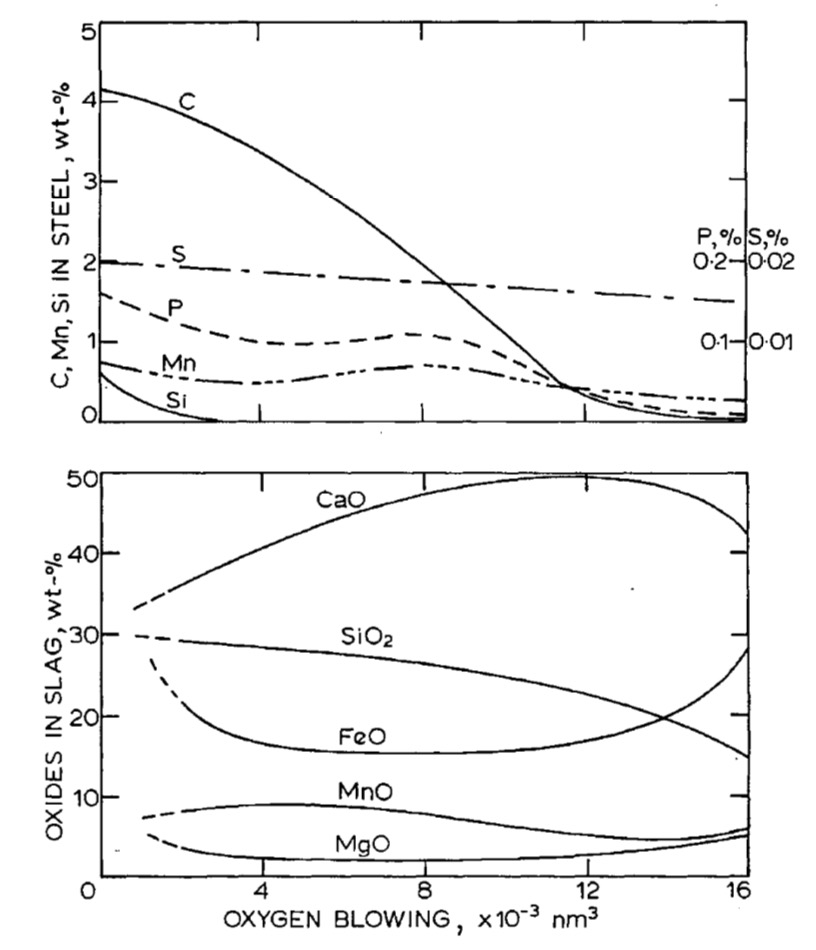
\includegraphics[width=.6\textwidth,angle=0]{slag-formation-data.jpg}
	\caption{Zmeny v zložení kovov a trosky počas výroby ocele v LD/BOF procesom pri 300t taveniny \citep{Turkdogan1996}.}
	\label{o:20}
\end{figure}

Intenzívny prúd kyslíka indukuje toky tekutín (cirkuláciu) v železnom kúpeli, následne núti vysoko oxidovaný kov a  roztavené oxidačné produkty z povrchu železného “kúpeľa” (iron bath) prenikať do vnútra kúpeľa, kde reagujú s “čerstvým” kovom s vysokým obsahom nečistôt. Tento prúd kyslíka a plynové bubliny vznikajúce v kúpeli privádzajú časti železnej taveniny do trosky. Teplo vyvíjané pri vysoko exotermálnych oxidačných reakciách sa spotrebúva pri zahrievaní a tavení vsádzkových materiálov, zahrievaní železného kúpeľa, trosky a oxidov uhlíka, ktoré sa tvoria pri oxidácii uhlíka a čiastočne sa strácajú do okolia počas procesu fúkania. Cirkulácie v železnom kúpeli spôsobené prúdom kyslíka, stúpajúcimi bublinami plynu a preplachovaním inertného plynu cez spodné trubice v kombinovaných vyfukovaných konvertoroch transportujú minoritné zložky taveniny železa (C, Si, Ti, Mn, P, V atď.) do horných vrstiev kúpeľa \cite{Jalkanen2006}. 

\begin{figure}[h!]
	\centering
	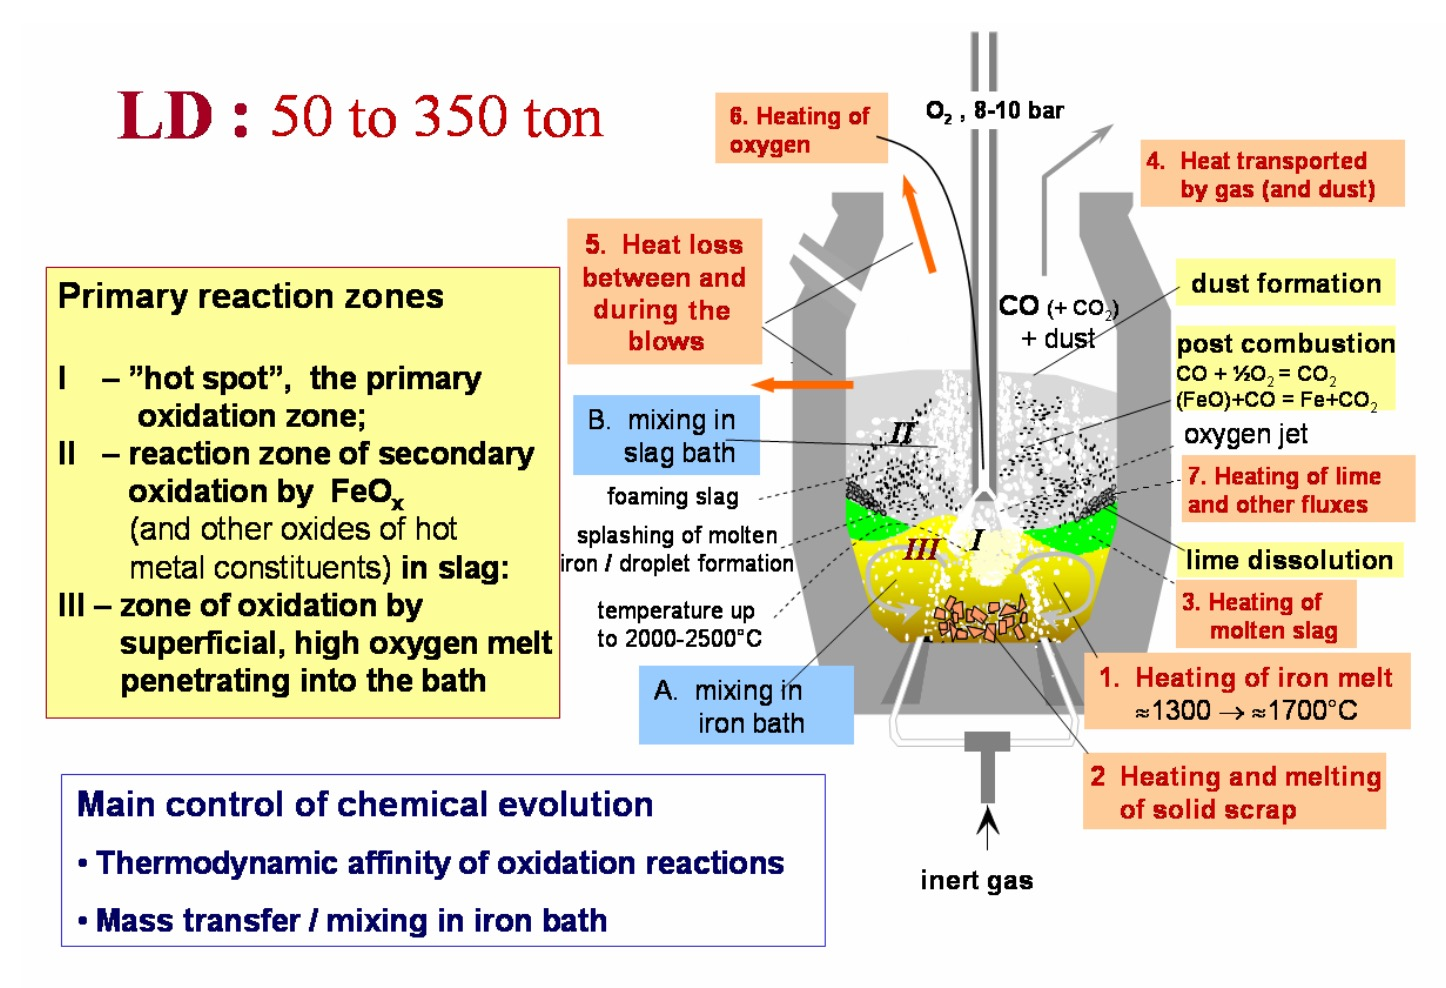
\includegraphics[width=.9\textwidth,angle=0]{ld-convertor-processes-graphical.jpg}
	\caption{Chemické a tepelné javy v LD konvertore \citep{Jalkanen2006}.}
	\label{o:25}
\end{figure}


\subsection{Riadenie procesov v kyslíkovom konvertore}

Keďže cieľom výroby oceli v kyslíkových konvertoroch je spálenie (tzv. oxidácia) nežiaducích nečistôt obsiahnutých v kovovej vsádzke, účelom tohto oxidačného procesu teda je:

\begin{itemize}
	\item znížiť obsah uhlíka na predpísanú úroveň (z približne 4 \% na menej ako 1 \%, ale často nižšie)
	\item upraviť obsah potrebných cudzích prvkov
	\item odstrániť nežiadúce nečistoty v maximálne možnej miere
\end{itemize}

Následnou úlohou riadiaceho procesu je potom získanie predpísaných parametrov pre oceľ, keď sa odoberá z pece, vrátane hmotnosti, teploty a obsahu každého prvku. Na základe týchto parametrov sa rozhoduje o tom, či je roztavená oceľ prijateľná alebo nie.

Počítačom podporované výpočty kontroly náboja sa robia pre každé teplo. Asi 80 percent modelu riadenia náboja je založené na rovnováhe tepla a materiálu, zvyšok je založený na empirických vzťahoch, ktoré sa medzi jednotlivými taviarňami líšia. Pretože každá oceliareň má svoju vlastnú formuláciu modelu regulácie náboja, v zjednodušenej forme sa tu bude diskutovať iba o všeobecných aspektoch tejto témy \cite{Turkdogan1996}.

Za účelom monitorovania a riadenia procesu je možné použiť rôzne meracie systémy na poskytnutie spätnej väzby operátorovi alebo priamo existujúcemu systému na automatizované riadenie. Tieto merania môžu byť priame alebo nepriame, ako aj s časovým oneskorením alebo bez neho \cite{Widlund1998}.

\begin{figure}[h!]
\centering
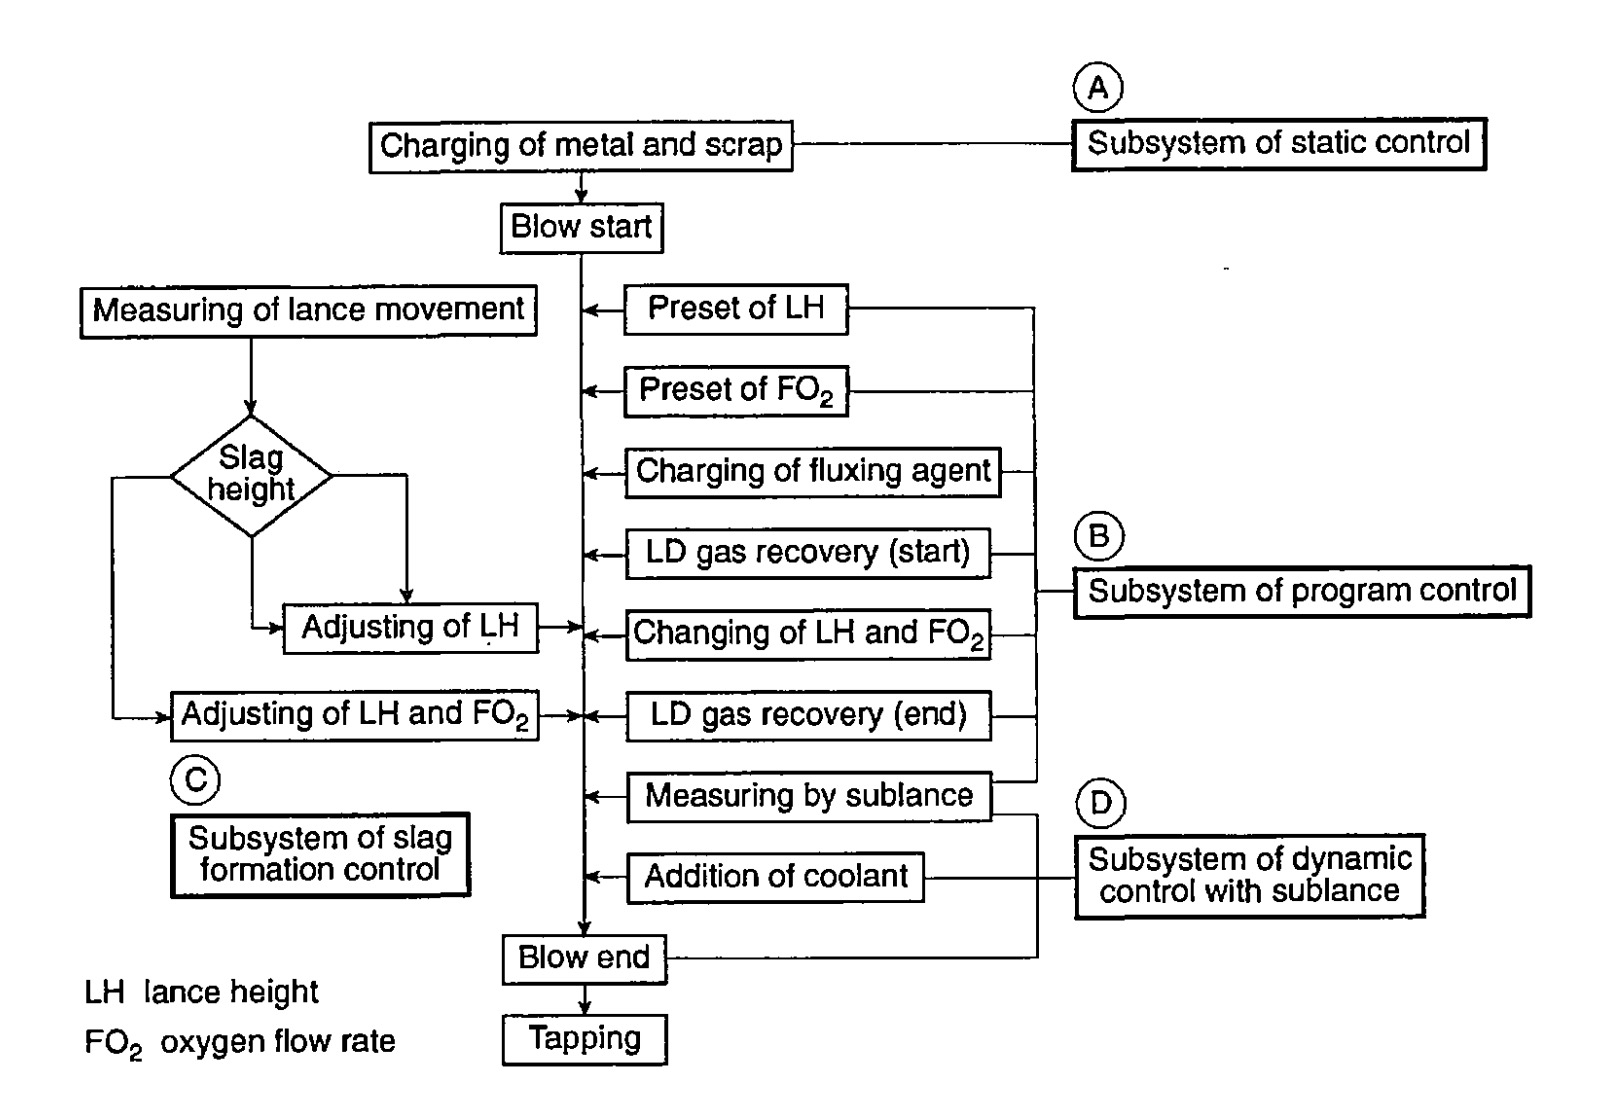
\includegraphics[width=.9\textwidth,angle=0]{schematic-bof.jpg}
\caption{Schéma funkcionality systému automatizovaného LD procesu \citep{Turkdogan1996}.}
\label{o:21}
\end{figure}

Existuje len niekoľko procesných premenných, ktoré môže manipulovať riadiaci systém alebo obsluha - výška trysky pre prívod fúkaného kyslíka, prietok kyslíka a prietok čistiaceho plynu. Zmeny vo výškach prívodnej trysky sa merajú a nastavujú ľahšie, a preto je lepšie ich používať v riadiacom systéme s uzavretou slučkou (closed-loop system). Zmena prietoku kyslíka počas LD procesu nesmie byť väčšia ako 5\%, pretože dýza je navrhnutá pre špecifický prietok. Naopak, prietok čistiaceho plynu sa môže meniť vo veľkom rozsahu \cite{Widlund1998}.